\documentclass{article}
\usepackage[scaled]{helvet}
\renewcommand\familydefault{\sfdefault}
\usepackage[T1]{fontenc}
\usepackage[utf8]{inputenc}
\usepackage[english]{babel}
\usepackage{graphicx}
\graphicspath{ {images/} }
\usepackage[all]{nowidow}
\usepackage{textcomp}
\usepackage{outlines}
\usepackage{listings}
\usepackage{spverbatim}
\usepackage{hyperref}

\usepackage[usenames, dvipsnames]{color}
\definecolor{logoblue}{RGB}{12, 27, 42}
\definecolor{logogreen}{RGB}{71, 82, 25}
\definecolor{successgreen}{RGB}{67, 160, 71}
\definecolor{failurered}{RGB}{229, 57, 53}


\setlength{\parindent}{4em}
\setlength{\parskip}{1em}


\widowpenalty10000
\clubpenalty10000

\begin{document}
\title{Using Panucci}
\maketitle
\begin{flushleft}
\section{What is Panucci?}
Panucci is a network-based testing and imaging platform, with a goal of simplifying the workflow of a computer buildout operation to make a single-piece flow viable and productive.
\pagebreak
\section{Intended workflow}
\begin{enumerate}
  \item Gather empty units for orders
  \item Grab a single unit
  \item Install HDD and RAM into unit
  \item Connect unit to server and input/output
  \item Power on unit
  \item Continue building and adding units as unit tests
  \item Upon test completion, begin imaging
  \item After imaging, verify correct boot
  \item Send unit to shipping
\end{enumerate}
\pagebreak
\section{Features}
\begin{itemize}
  \item Single workflow for all units
  \item Built-in partitioning and image creation
  \item Software allows for adding modular hardware
  \item HDD Testing (using \verb|smartctl| and \verb|seeker|)
  \begin{itemize}
    \item Linear Write Speed
    \item Linear Read Speed
    \item SMART Short Self-Test
    \item SMART Health Check
    \item Random Seek Test
  \end{itemize}
  \item RAM testing using \verb|memtester|
  \item Automatic integration with SellerCloud using the \verb|ScrubDeku| gem
  \item Support for label printing
  \item Basic logging, with upcoming support for a database logging system
  \item Used with \verb|Seymour|, a script for creating a full image tree off of one image
  \item Simple interface built on CSS and HTML, allowing easy modification and updating
\end{itemize}
\pagebreak
\section{Basic Use}
This section assumes you have already created a working PXE server for Panucci, and are able to boot into it.  See document "Creating A PXE Server" for information on this.  These instructions assume your existing setup followed the same basic setup as that detailed in "Creating a PXE Server".
\subsection{Starting the server}
The server for Panucci can simply be powered on.  As long as there are no errors, it will automatically begin serving up the needed files.
\subsection{Booting Panucci}
To begin using Panucci, after building out a unit with RAM and HDD, connect it to appropriate network port and power it on.  Assuming a blank drive, network boot should be automatic as long as the unit supports it.
\subsection{Testing in Panucci}
Testing begins automatically on boot.  Users can monitor testing on the displayed status.

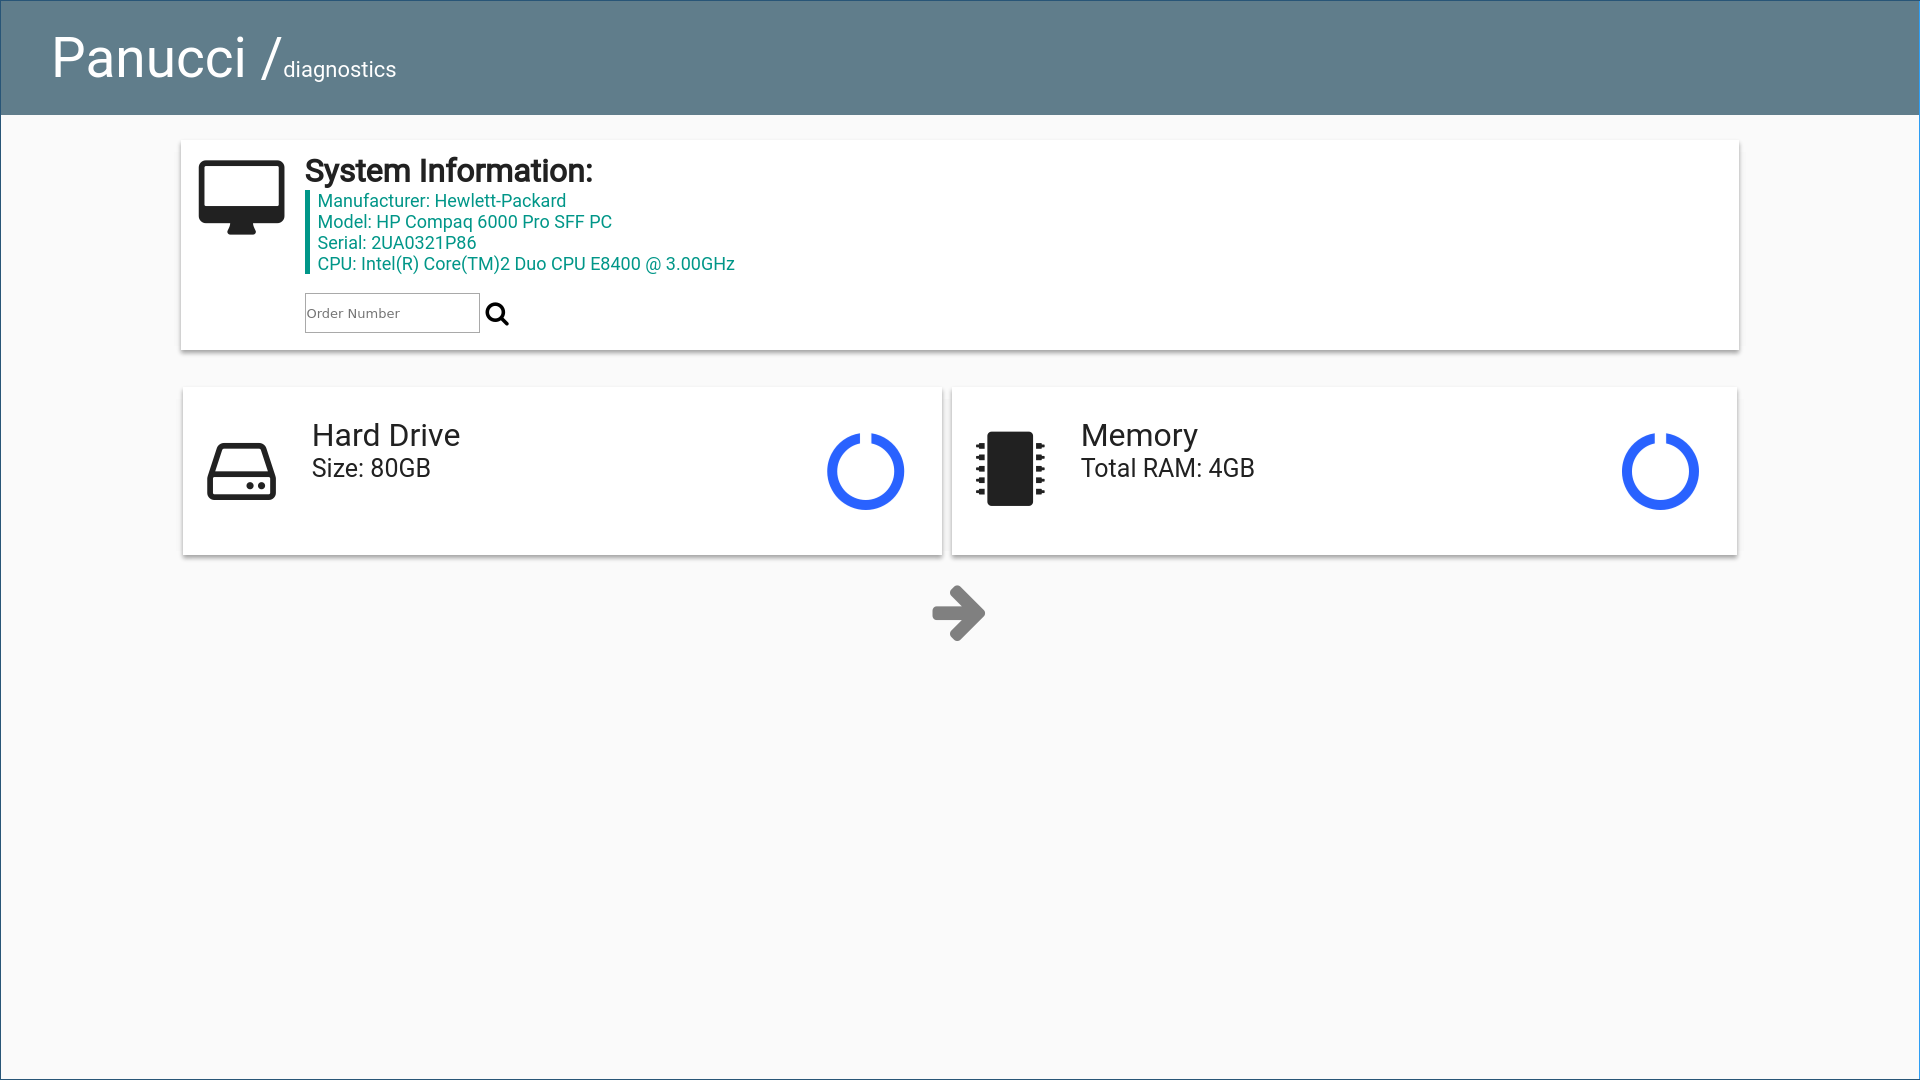
\includegraphics[width=\textwidth]{testing_view}

\subsection{Order Verification}
Panucci supports order verification using SellerCloud.  To verify an order, click inside the order number entry box.

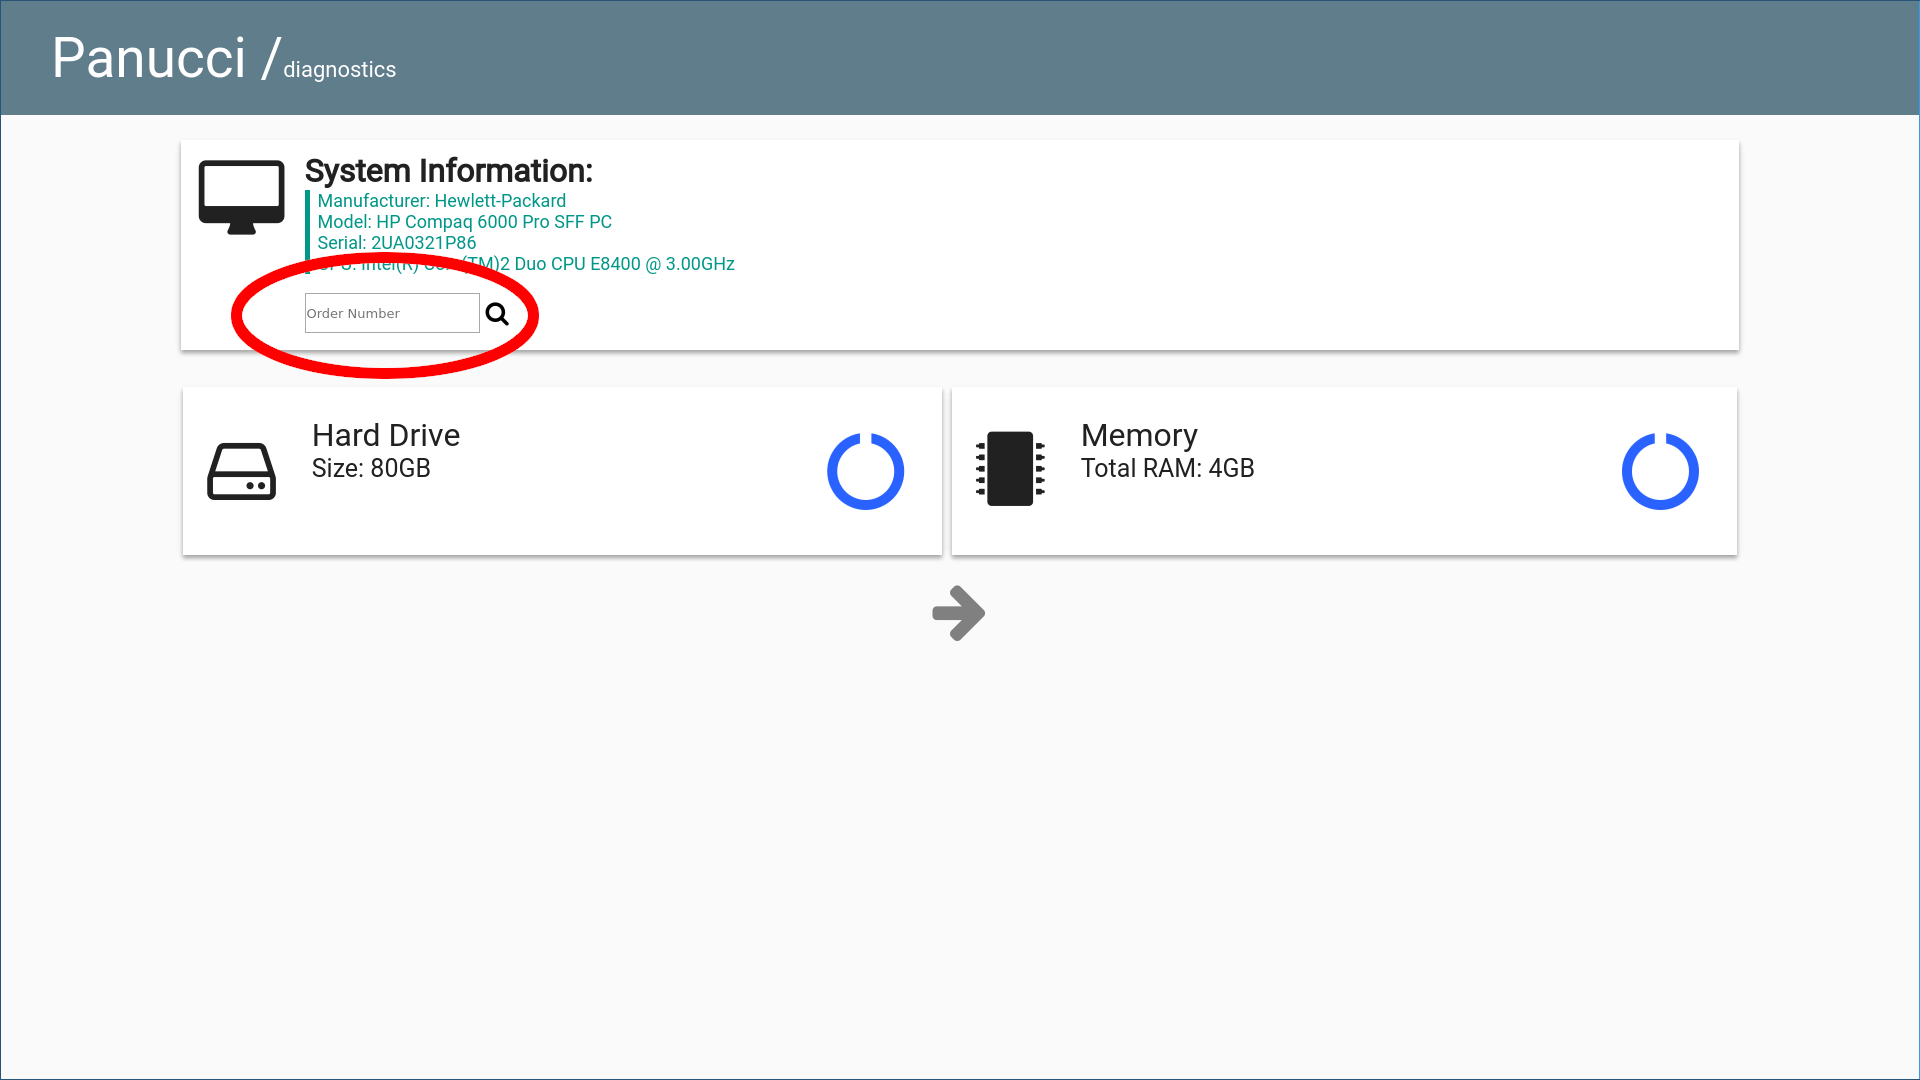
\includegraphics[width=\textwidth]{order_box}

After entering the order number, click the magnifying glass icon to search for the order.  Orders with multiple computer kits will redirect to a page with all options; select the correct option to proceed.

After getting the order data, the testing page will contain the relevant order data, as well as visual indicators.  \textcolor{successgreen}{Green or Checkmarks} mean the unit matches the order; \textcolor{failurered}{Red or Xs} mean the unit does not match the order.

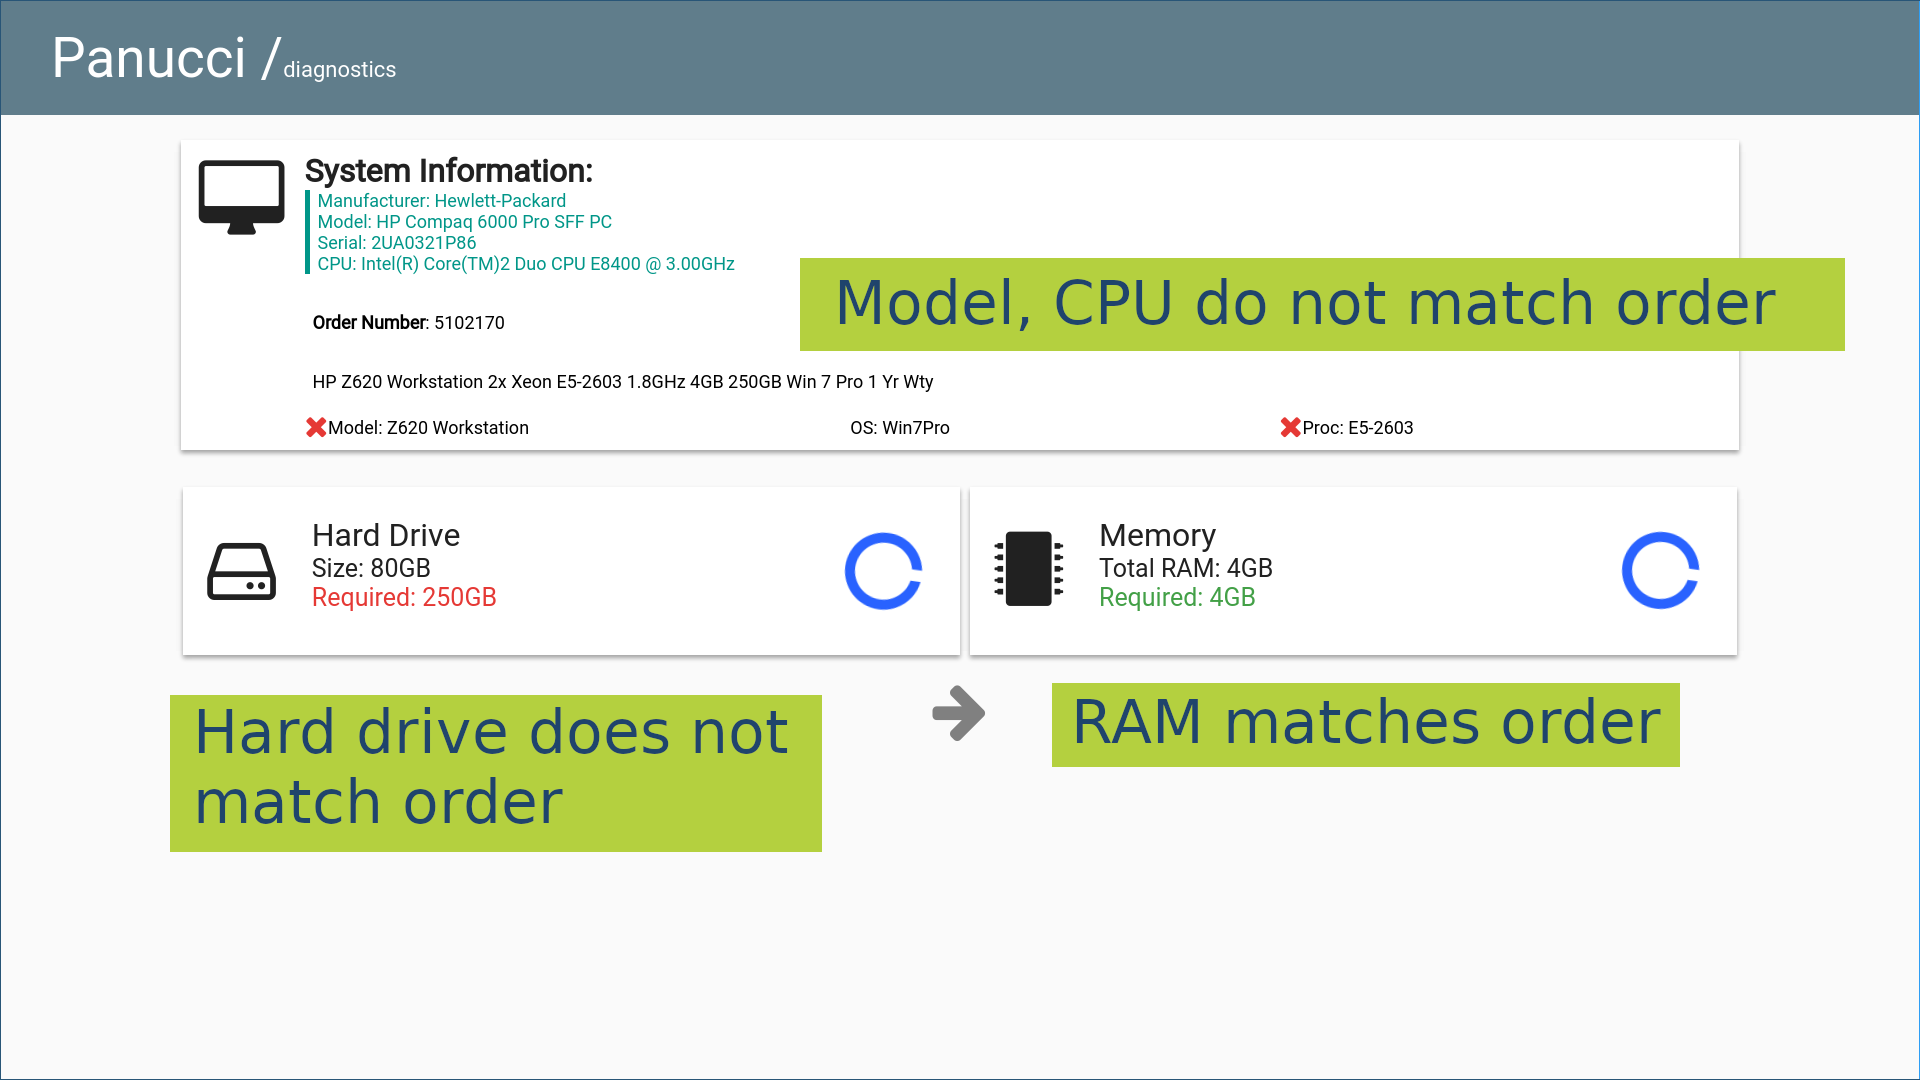
\includegraphics[width=\textwidth]{verification_note}

In the above example, HDD capacity, Model, and Proc are all different from the order, as noted by the \textcolor{failurered}{red text and Xs}.  Only the RAM matches, as noted by the \textcolor{successgreen}{green text}.
\subsection{Proceeding after success}
After testing has completed, a label will print out, regardless of pass or fail.  If the unit has passed, the green arrow at the bottom will become available:

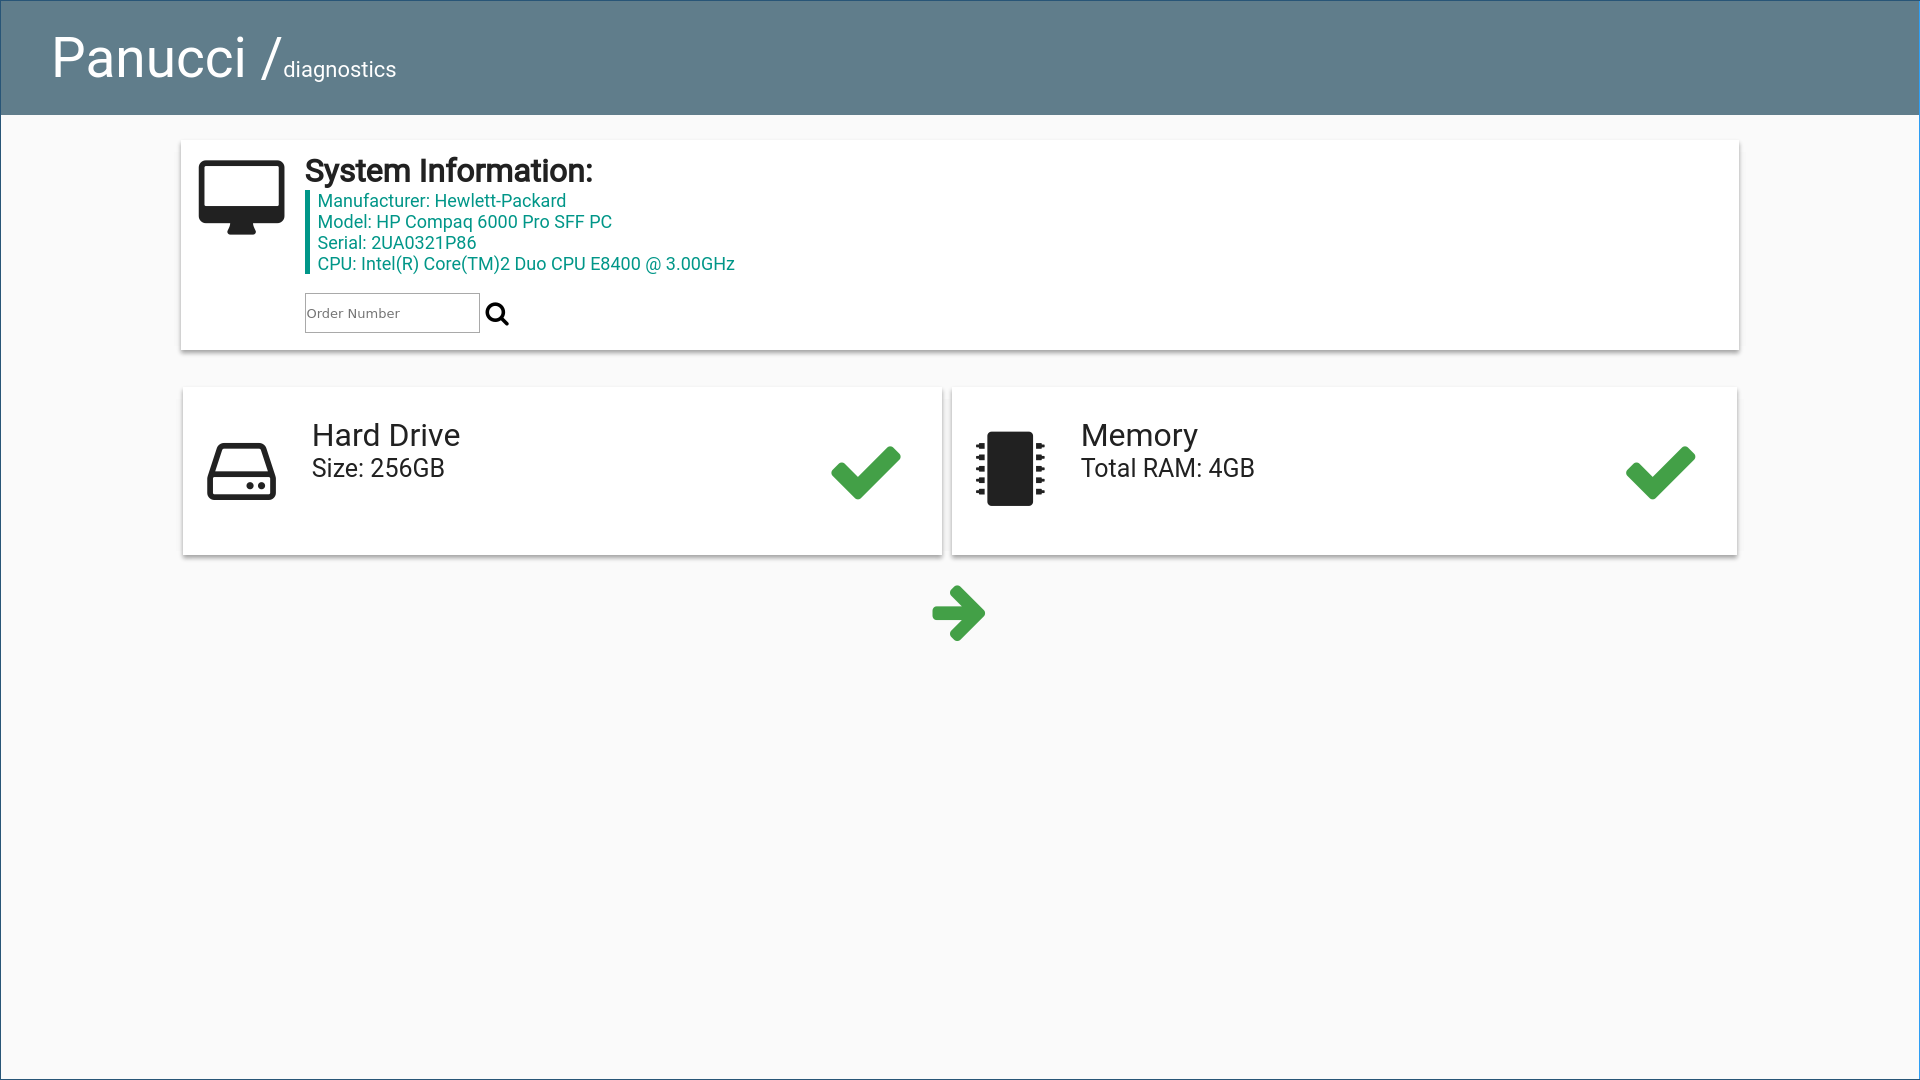
\includegraphics[width=\textwidth]{test_good}

Click the green arrow to begin the imaging process.  If the unit didn't pass all tests, fix the problems and re-test the machine.

\subsection{Imaging in Panucci}

After testing is completed and clicking the green arrow to proceed, a prompt appears to see if the unit is to be imaged with Windows 10.

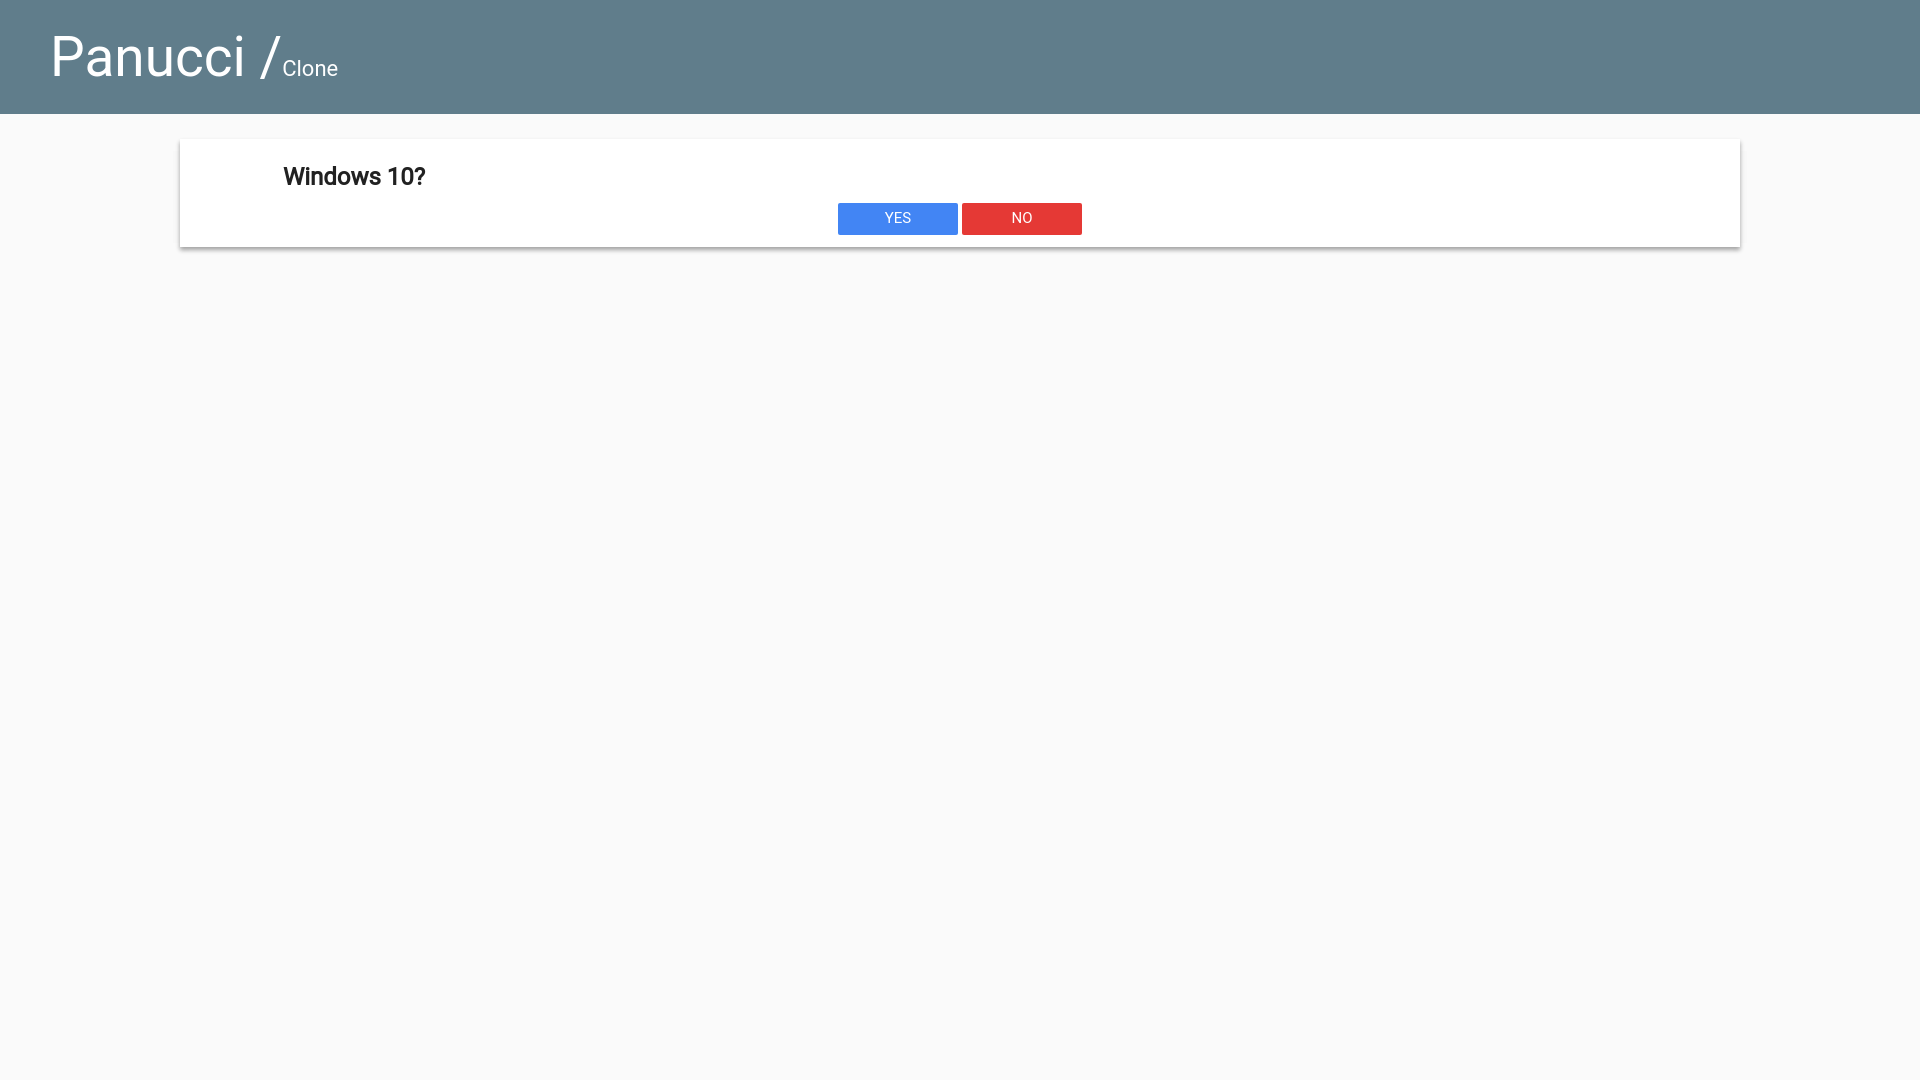
\includegraphics[width=\textwidth]{win10}

Clicking yes will immediately ask you to confirm to image with Windows 10, with the size detected by Panucci.  Confirm to begin imaging with Windows 10.

If you select no, you will be taken to an image selection tree.

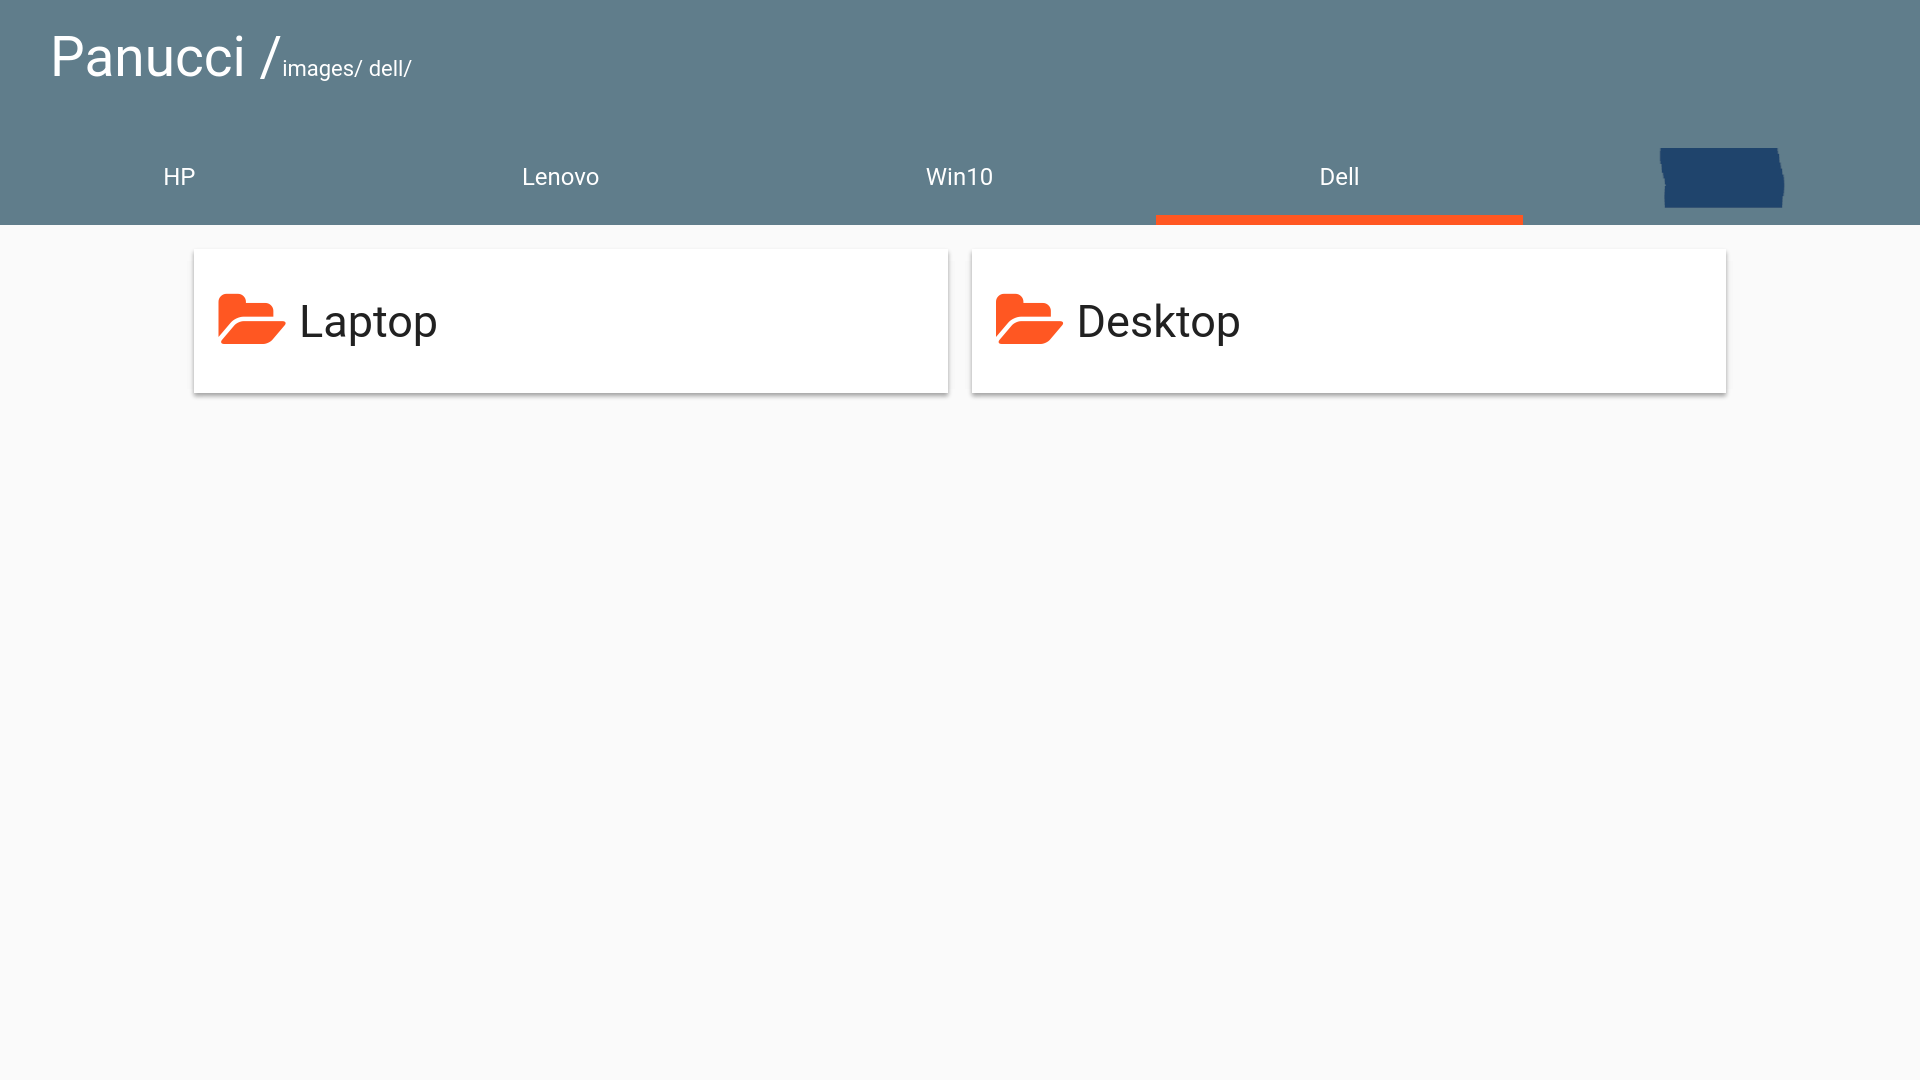
\includegraphics[width=\textwidth]{folder_view}

To navigate the tree, select a manufacturer at the top by clicking on it.  Once a manufacturer has been selected, work through the tree by click on the appropriate label.  Once a directory that contains images has been selected, Panucci will prompt to confirm imaging with the selected model and size.  Confirm to image, deny to return to image selection.
\end{flushleft}
\end{document}
